\section{Configuration}

\subsection{General}

The general configuration allows the user to enter a identification. Also the user can
specify where will the program store the auto-save files and how often will the program
backup the ongoing session.

\begin{figure}[H]
\centering
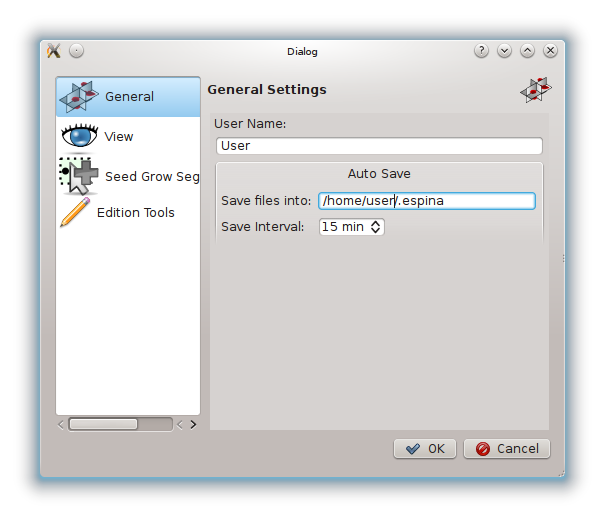
\includegraphics[scale=0.75]{fig/Configuration-general}
\caption{General configuration widget.}
\end{figure}

\subsection{View}

The view configuration offer the posibility of inverting the slice order in each of the
planar views, reversing the stack only for that view, and to invert the use of the mouse
wheel. \\
For the three-dimensional view, the renderers can be marked as active (meaning the
three-dimensional view will add a button to enable/disable that representations) or available
(won't appear on the renderers list in the 3D view widget).
\vspace{0.3cm}

\begin{bclogo}[couleur = yellow!33, logo=\bcattention]
{Note} Plugins can add their own renderers. Refer to the plugin documentation for more information.
When a renderer is added it is by default marked as ``Available''.
\end{bclogo}

\begin{figure}[H]
\centering
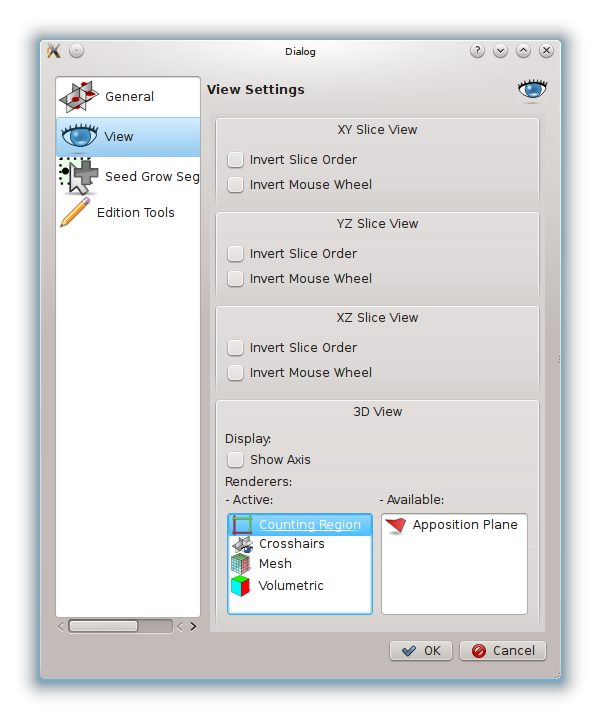
\includegraphics[scale=0.75]{fig/Configuration-view}
\caption{View configuration widget.}
\end{figure}

\subsection{Seed grow segmentation}

The value of the ``best pixel'' used in the seed grow segmentation algorithm can be configured using
a slider that goes from a complete black value to a complete white one. Also the size of the ``volume
of interest'' can be defined by giving the length of each of it's sides.\\
Once the seed algorithm has obtained a segmentation usually the user applies a closing algorithm to
make it compact. The option to make this step automatic can be configured here, with the possibility of
specifying the radius of the structuring element of the closing algorithm.\\

\begin{figure}[H]
\centering
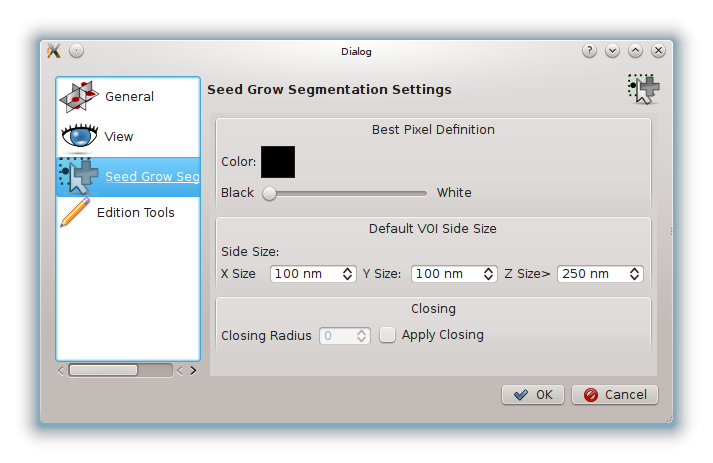
\includegraphics[scale=0.75]{fig/Configuration-seed}
\caption{Seed grow segmentation configuration widget.}
\end{figure}

\subsection{Edition tools}

The radius of the paint and erase brushes can be configured in screen pixels. Also the structuring element
radius of the morphological filters can be defined. \\

\begin{figure}[H]
\centering
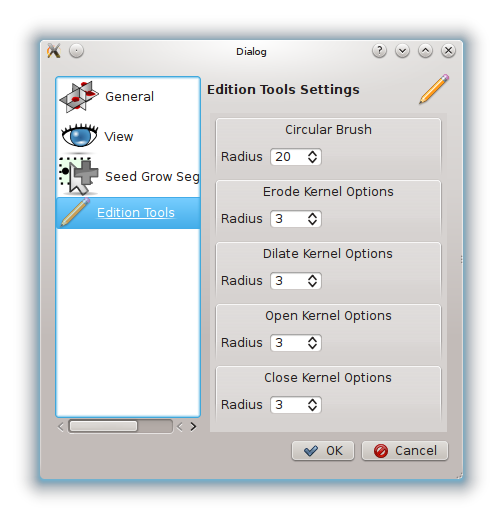
\includegraphics[scale=0.65]{fig/Configuration-edit}
\caption{Edition tools configuration widget.}
\end{figure}

